\chapter{Related Work}
\label{cha:relatedwork}

The state of the art goes here. This includes:
\begin{itemize}
    \item an overview over available technology
    \item a dicussion which technology is best to use
    \item CISCO MSE API wrapper test results
\end{itemize}


\vspace{0.5cm}

We are now going to take a look into what technology is available to accomplish our project goals defined in the previous chapter. First, we are starting with an overview of localization technologies that are in the reach of our project. After that we evaluate which ones are suitable for the circumstances our project is positioned in. And at the end one specific available solution will be examined more deeply in order to determine its possible value for our implementation.


\vspace{0.5cm}

\section{Projects With Same Idea}


\vspace{0.5cm}

\section{Localization Technologies}


\vspace{0.5cm}

\section{Evaluation of Available Technologies}


\vspace{0.5cm}

\section{CISCO MSE API Wrapper Tests}

In order to determine whether the CISCO MSE API wrapper provided by tubIT would be sufficient for the project's requirements we were asked to perform tests on it. Especially it was asked for details on how the API worked where, so what values could be retrieved via the API wrapper in which locations on campus and how precise the values would turn out to be.

Concerning use cases our project was focused on the mensa and the library, therefore we initially planned to be conducting tests in only these two locations. As the provided wrapper around the CISCO MSE API we had access to delivered back one short, simple XML line we decided to invest some time into developing a small tool which routinely queried the API for it's current status and saved the result into an easily readable JSON file for later investigation. The source code of the developed tool you can find in appendix \ref{appendix:cisco-mse-api-test}.

\begin{center}
    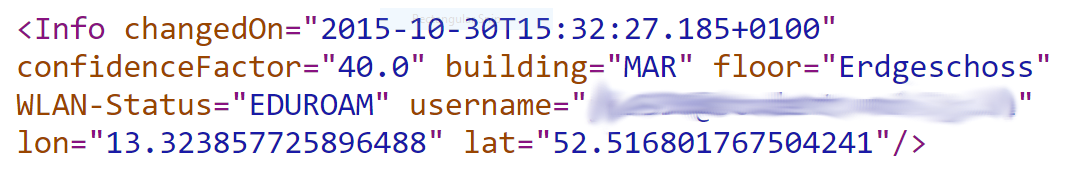
\includegraphics[width=\textwidth]{cisco-mse-api-response}\\
    What the CISCO MSE API wrapper response looks like.
\end{center}

It was planned to be conducting the tests on one day in the mensa and on another day in the library. On the first day we started around noon and ran the test tool on one of our notebooks connected to university WiFi, \enquote{eduroam}. We started in the south-western corner near the windows, walked towards the south-eastern corner, went to the stairs in the northern part and upstairs and again at the window front to the south-western corner on the first floor. As it turned out, the results we got back were definitely not what we had hoped for, most importantly because longitude and latitude of the requesting user were missing completely. The following listing shows the first ten results logged in two second periods from the API wrapper:

\begin{lstlisting}
{
    "signal": [
        {"timestamp": 1445344391, "latitude": "0.000000000000000", "longitude": "0.000000000000000", "building": "Mensa", "floor": "Mensa 1. OG"},
        {"timestamp": 1445344393, "latitude": "0.000000000000000", "longitude": "0.000000000000000", "building": "Mensa", "floor": "Mensa 1. OG"},
        {"timestamp": 1445344395, "latitude": "0.000000000000000", "longitude": "0.000000000000000", "building": "Mensa", "floor": "Mensa 1. OG"},
        {"timestamp": 1445344397, "latitude": "0.000000000000000", "longitude": "0.000000000000000", "building": "Mensa", "floor": "Mensa 1. OG"},
        {"timestamp": 1445344399, "latitude": "0.000000000000000", "longitude": "0.000000000000000", "building": "Mensa", "floor": "Mensa 1. OG"},
        {"timestamp": 1445344401, "latitude": "0.000000000000000", "longitude": "0.000000000000000", "building": "Mensa", "floor": "Mensa 1. OG"},
        {"timestamp": 1445344404, "latitude": "0.000000000000000", "longitude": "0.000000000000000", "building": "Mensa", "floor": "Mensa 1. OG"},
        {"timestamp": 1445344406, "latitude": "0.000000000000000", "longitude": "0.000000000000000", "building": "Mensa", "floor": "Mensa 1. OG"},
        {"timestamp": 1445344408, "latitude": "0.000000000000000", "longitude": "0.000000000000000", "building": "Mensa", "floor": "Mensa 1. OG"},
        {"timestamp": 1445344410, "latitude": "0.000000000000000", "longitude": "0.000000000000000", "building": "Mensa", "floor": "Mensa 1. OG"},
        ...
    ]
}
\end{lstlisting}

Clearly it can be observed that the longitude and latitude values are unusable. Another take away was that the floor change during our test did not reflect into our captured results. Therefore we decided to directly test the library for comparable results. Inside the library, we started on ground floor and went upstairs in \enquote{circles} through the different levels. From the fourth floor we went back down straight forward. During that second test ten of the first fifteen responses from the API looked like:

\begin{lstlisting}
{
    "signal": [
        {"timestamp": 1445345843, "latitude": "0.000000000000000", "longitude": "0.000000000000000", "building": "BIB", "floor": "Erdgeschoss"},
        {"timestamp": 1445345845, "latitude": "0.000000000000000", "longitude": "0.000000000000000", "building": "BIB", "floor": "Erdgeschoss"},
        {"timestamp": 1445345848, "latitude": "0.000000000000000", "longitude": "0.000000000000000", "building": "BIB", "floor": "Erdgeschoss"},
        {"timestamp": 1445345850, "latitude": "0.000000000000000", "longitude": "0.000000000000000", "building": "BIB", "floor": "Erdgeschoss"},
        {"timestamp": 1445345852, "latitude": "0.000000000000000", "longitude": "0.000000000000000", "building": "BIB", "floor": "Erdgeschoss"},
        {"timestamp": 1445345854, "latitude": "0.000000000000000", "longitude": "0.000000000000000", "building": "BIB", "floor": "Erdgeschoss"},
        ...
        {"timestamp": 1445345870, "latitude": "0.000000000000000", "longitude": "0.000000000000000", "building": "BIB", "floor": "1. Obergeschoss"},
        {"timestamp": 1445345872, "latitude": "0.000000000000000", "longitude": "0.000000000000000", "building": "BIB", "floor": "1. Obergeschoss"},
        {"timestamp": 1445345874, "latitude": "0.000000000000000", "longitude": "0.000000000000000", "building": "BIB", "floor": "1. Obergeschoss"},
        {"timestamp": 1445345876, "latitude": "0.000000000000000", "longitude": "0.000000000000000", "building": "BIB", "floor": "1. Obergeschoss"},
        ...
    ]
}
\end{lstlisting}

First, longitude and latitude were again unusable. This time though the floor information worked quite reliably and indicated very fast on which floor we currently measured. After that we were wondering whether eventually we would get back longitude and latitude values anywhere on campus and decided to give it one last try by taking one more measurement in the MAR building (Marchstraße).

One more measurement turned into three as during the first two attempts we got sudden disconnects and therefore unusable results. We walked the whole foyer from north to south side and somewhere near the entrance we suspect the wireless signal got bad and our notebook conducting the tests disconnected. In the third try though we finally were able to get back usable results, in which chosen ten results logged looked like this:

\begin{lstlisting}
{
    "signal": [
        {"timestamp": 1445350550, "latitude": "52.516903688639005", "longitude": "13.323958376544699", "building": "MAR", "floor": "Erdgeschoss"},
        {"timestamp": 1445350552, "latitude": "52.516903688639005", "longitude": "13.323958376544699", "building": "MAR", "floor": "Erdgeschoss"},
        {"timestamp": 1445350554, "latitude": "52.516903688639005", "longitude": "13.323958376544699", "building": "MAR", "floor": "Erdgeschoss"},
        {"timestamp": 1445350557, "latitude": "52.516903688639005", "longitude": "13.323958376544699", "building": "MAR", "floor": "Erdgeschoss"},
        ...
        {"timestamp": 1445350686, "latitude": "52.516864921942748", "longitude": "13.323953890659670", "building": "MAR", "floor": "Erdgeschoss"},
        {"timestamp": 1445350688, "latitude": "52.516864921942748", "longitude": "13.323953890659670", "building": "MAR", "floor": "Erdgeschoss"},
        {"timestamp": 1445350690, "latitude": "52.516864921942748", "longitude": "13.323953890659670", "building": "MAR", "floor": "Erdgeschoss"},
        ...
        {"timestamp": 1445350845, "latitude": "52.516402095317481", "longitude": "13.323531401046099", "building": "MAR", "floor": "Erdgeschoss"},
        {"timestamp": 1445350847, "latitude": "52.516402095317481", "longitude": "13.323531401046099", "building": "MAR", "floor": "Erdgeschoss"},
        {"timestamp": 1445350849, "latitude": "52.516402095317481", "longitude": "13.323531401046099", "building": "MAR", "floor": "Erdgeschoss"},
        ...
    ]
}
\end{lstlisting}

Finally we received some longitude and latitude values. Unfortunately the three different pairs of longitude and latitude above were the only ones we could observe during the whole walk from north end to south end of the foyer, thus still rather unusable values.

In the end, our conclusion at that point in the project progress was to use the CISCO MSE API wrapper provided by the tubIT in order to retrieve the rough position of a user. This means the building and floor the request originated from. We recommended back to our supervisors not to use this API for receiving longitude and latitude as these values were either quite imprecise or not available at all. The full result files of all our three measurements can be found at \cite{ioslINavGitHub}.